% ----- Fonctionnement -----

\subsection{How it works}

    To explain how our algorithm works, we will keep track of two groups of vertices : $S$ which is a partially constructed clique and the partial solution that we will gradually implement. Moreover, we also have $Z$ which is the list of all the vertices sorted according to a criterion (the best degree). Furthermore, we got $P$  which is the candidates vertices that could be included in the clique, and which represents the union of all vertex neighbors of the vertices in $S$.
    \\ \\
    The algorithm begins by forming a list of all the vertices sorted according to a criterion (the best degree). This is to facilitate the identification of the next vertices that we will add to our solution $S$. This makes it easier to identify the next vertices to be added to our solution $S$, it also saves complexity because we are not bound to check each criterion at each iteration. Then the algorithm will initialize $P$, and insert in it all the vertices of the graph.
    \\ \\
    It will then retrieve the first element of the list $Z$ that also belongs to $P$, and add it to the solution $S$. The selected element will then be removed from $Z$. After this step, $P$ is updated by considering only the neighbors of the vertices that are already part of $S$. This process is then repeated recursively until no more vertices are left in $P$, at which point the algorithm has obtained its maximum clique $S$.
    \\ \\
    To illustrate the Constructive algorithm, let's use the example in
    Figure \ref{fig:basic-graph-example} on page \pageref{fig:basic-graph-example} while adding some weight to its edges: \\

    \begin{minipage}{\linewidth}
        \textbf{Step 0:} \newline
        \begin{minipage}{0.4\textwidth}
            \begin{figure}[H]
                \centering
                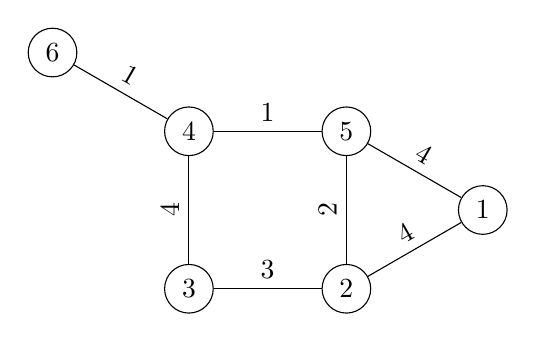
\begin{tikzpicture}[node distance=2cm]
                    \node[circle, draw] (1) {1};
                    \node[circle, draw] (2) at ([shift=(210:2)] 1) {2};
                    \node[circle, draw] (3) [left of=2] {3};
                    \node[circle, draw] (4) [above of=3] {4};
                    \node[circle, draw] (5) [above of=2] {5};
                    \node[circle, draw] (6) at ([shift=(150:2)] 4) {6};
    
                    \draw  (1) -- (2) node[midway, above, sloped] {4};
                    \draw (1) -- (5) node[midway, above, sloped] {4};
                    \draw (2) -- (3) node[midway, above, sloped] {3};
                    \draw (2) -- (5) node[midway, above, sloped] {2};
                    \draw (3) -- (4) node[midway, above, sloped] {4};
                    \draw (4) -- (5) node[midway, above, sloped] {1};
                    \draw (4) -- (6) node[midway, above, sloped] {1};
                \end{tikzpicture}
                \caption{Graph illustration for the constructive algorithm at step 0}
                \label{fig:constructive-mewc-maxedge-step0}
            \end{figure}
        \end{minipage}
        \begin{minipage}{0.6\textwidth}
            At the initial step, as said before, we will initialize $S$, $P$ and $Z$ by sorting the vertices based on a criterion. Here we chose the vertex of the highest degree.
            \begin{center}
                \begin{tabular}{|lll|}
                    \hline
                    S = \{$\emptyset$\} & P = \{1,2,3,4,5,6\} & Z = \{2,4,5,1,3,6\} \\
                    \hline
                \end{tabular}
            \end{center}
        \end{minipage}
    \end{minipage} 
    
    \vspace{1\baselineskip}

    \begin{minipage}{\linewidth}
        \textbf{Step 1:} \newline
        \begin{minipage}{0.4\textwidth}
            \begin{figure}[H]
                \centering
                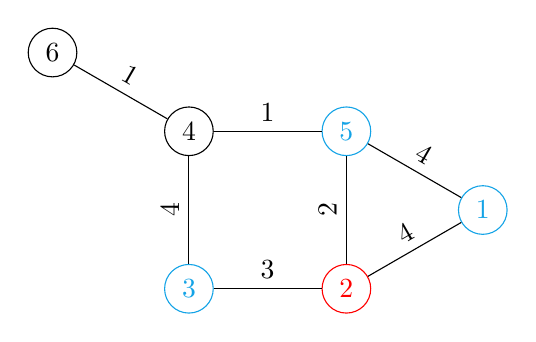
\begin{tikzpicture}[node distance=2cm]
                    \node[circle, draw, Cerulean] (1) {1};
                    \node[circle, draw, Red] (2) at ([shift=(210:2)] 1) {2};
                    \node[circle, draw, Cerulean] (3) [left of=2] {3};
                    \node[circle, draw] (4) [above of=3] {4};
                    \node[circle, draw, Cerulean] (5) [above of=2] {5};
                    \node[circle, draw] (6) at ([shift=(150:2)] 4) {6};
    
                    \draw  (1) -- (2) node[midway, above, sloped] {4};
                    \draw (1) -- (5) node[midway, above, sloped] {4};
                    \draw (2) -- (3) node[midway, above, sloped] {3};
                    \draw (2) -- (5) node[midway, above, sloped] {2};
                    \draw (3) -- (4) node[midway, above, sloped] {4};
                    \draw (4) -- (5) node[midway, above, sloped] {1};
                    \draw (4) -- (6) node[midway, above, sloped] {1};
                \end{tikzpicture}
                \caption{Graph illustration for the constructive algorithm at step 1}
                \label{fig:constructive-mewc-maxedge-step1}
            \end{figure}
        \end{minipage}
        \begin{minipage}{0.6\textwidth}
            In step 1, the algorithm will take the first vertex of $Z$ if it is common to $P$ (here 2). In case of a tie, the algorithm will take the first checked vertex. He will then add it to $S$, represented in \textcolor{red}{red}. $P$, represented in \textcolor{Cerulean}{blue}, will be updated by taking only the vertices that are neighbors to all the members of $S$ (here, $S$ is composed only of vertex 2, so we take only the neighbors of 2).
    
            \begin{center}
                \begin{tabular}{|lll|}
                    \hline
                    S = \{2\} & P = \{3,5,1\} & Z = \{4,5,1,3,6\} \\
                    \hline
                \end{tabular}
            \end{center}
        \end{minipage}
    \end{minipage} 

    \vspace{1\baselineskip}

    \begin{minipage}{\linewidth}
        \textbf{Step 2:} \newline
        \begin{minipage}{0.4\textwidth}
            \begin{figure}[H]
                \centering
                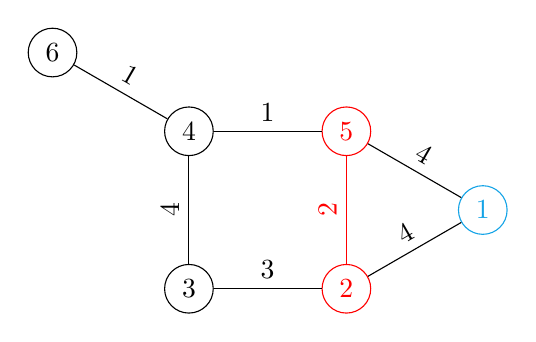
\begin{tikzpicture}[node distance=2cm]
                    \node[circle, draw, Cerulean] (1) {1};
                    \node[circle, draw, red] (2) at ([shift=(210:2)] 1) {2};
                    \node[circle, draw] (3) [left of=2] {3};
                    \node[circle, draw] (4) [above of=3] {4};
                    \node[circle, draw, red] (5) [above of=2] {5};
                    \node[circle, draw] (6) at ([shift=(150:2)] 4) {6};
    
                    \draw  (1) -- (2) node[midway, above, sloped] {4};
                    \draw (1) -- (5) node[midway, above, sloped] {4};
                    \draw (2) -- (3) node[midway, above, sloped] {3};
                    \draw[red] (2) -- (5) node[midway, above, sloped] {2};
                    \draw (3) -- (4) node[midway, above, sloped] {4};
                    \draw (4) -- (5) node[midway, above, sloped] {1};
                    \draw (4) -- (6) node[midway, above, sloped] {1};
                \end{tikzpicture}
                \caption{Graph illustration for the constructive algorithm at step 2}
                \label{fig:constructive-mewc-edge-step2}
            \end{figure}
        \end{minipage}
        \begin{minipage}{0.6\textwidth}
            In step 2, the algorithm will repeat the process of step 1 by making a recursive call until $P$ is empty. We can note in the process that our algorithm iterates again on some elements of $Z$, deleting them and refactoring the list does not improve the complexity, but implementing it as we did improve it in general(by not checking every neighbors each times). 
    
            \begin{center}
                \begin{tabular}{|lll|}
                    \hline
                    S = \{2,5\} & P = \{1\} & Z = \{4,1,3,6\} \\
                    \hline
                \end{tabular}
            \end{center}
        \end{minipage}
    \end{minipage}

    \vspace{1\baselineskip}

    \begin{minipage}{\linewidth}
        \textbf{Step 3:} \newline
        \begin{minipage}{0.4\textwidth}
            \begin{figure}[H]
                \centering
                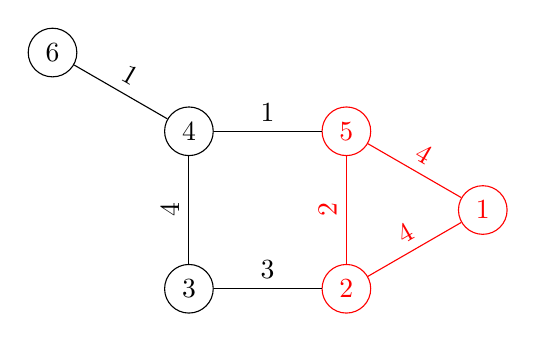
\begin{tikzpicture}[node distance=2cm]
                    \node[circle, draw, red] (1) {1};
                    \node[circle, draw, red] (2) at ([shift=(210:2)] 1) {2};
                    \node[circle, draw] (3) [left of=2] {3};
                    \node[circle, draw] (4) [above of=3] {4};
                    \node[circle, draw, red] (5) [above of=2] {5};
                    \node[circle, draw] (6) at ([shift=(150:2)] 4) {6};
    
                    \draw[red]  (1) -- (2) node[midway, above, sloped] {4};
                    \draw[red] (1) -- (5) node[midway, above, sloped] {4};
                    \draw (2) -- (3) node[midway, above, sloped] {3};
                    \draw[red] (2) -- (5) node[midway, above, sloped] {2};
                    \draw (3) -- (4) node[midway, above, sloped] {4};
                    \draw (4) -- (5) node[midway, above, sloped] {1};
                    \draw (4) -- (6) node[midway, above, sloped] {1};
                \end{tikzpicture}
                \caption{Graph illustration for the constructive algorithm at step 3}
                \label{fig:constructive-mewc-edge-step3}
            \end{figure}
        \end{minipage}
        \begin{minipage}{0.6\textwidth}
            In step 3, the algorithm repeat the step 1 by making a recursive call. It will finally find 1 which is the last vertex of $P$. The algorithm stop, and we get the maximum clique in \textcolor{red}{red} $(1,2,5)$.
    
            \begin{center}
                \begin{tabular}{|lll|}
                    \hline
                    S = \{2,5,1\} & P = \{\} & Z = \{4,3,6\} \\
                    \hline
                \end{tabular}
            \end{center}
        \end{minipage}
    \end{minipage}


\vspace{1\baselineskip}

    Now we calculate the weight of this clique. The constructive algorithm is now finished, and we have obtained the following maximum clique of weight 10 : $$(1,2,5)$$

\newpage

